\documentclass{beamer}

\mode<presentation> {
  \usetheme{CambridgeUS}
  \setbeamercovered{transparent}
}

%\usepackage[latin2]{inputenc}
\usepackage[slovak]{babel}
\usepackage[utf8]{inputenc}
\usepackage{amsmath,amssymb}
\usepackage{graphicx}
\usepackage{caption}
%\newcommand{\ml}{l\kern-0.035cm\char39\kern-0.03cm}
%\newcommand{\mt}{t\kern-0.035cm\char39\kern-0.03cm}
%\newcommand{\md}{d\kern-0.035cm\char39\kern-0.03cm}
\title{Triangulárne normy (t-normy)}
\author{Martin Bažík, Milan Augustín, Ľuboš Hlipala}

\begin{document}
\begin{frame}
	\maketitle
\end{frame}
%\begin{frame}
%  \frametitle{Osnova}
%  \tableofcontents
%\end{frame}

\begin{frame}
  \frametitle{T-normy}
  \begin{definition}
  	\textbf{Binárna operácia} na intervale [0,1], t.j. funkcia $T : [0,1]^2 \rightarrow [0,1]$ splňujúca axiómy:
  	\begin{itemize}
  		\item (T1) {\em Komutatívnosť}
		$T(x,y)=T(y,x)$
		\item (T2) {\em Asociatívnosť}
		$T(x,T(y,z))=T(T(x,y),z)$
		\item (T3) {\em Monotónnosť}
		$ ak \hskip 2mm y\le z, \hskip 2mm tak \hskip 2mm T(x,y)\le T(x,z)$
		\item (T4) {\em Okrajová podmienka}
		$T(x,1)=x.$
	\end{itemize}
  \end{definition}
  \begin{itemize}
  	\item Fuzzy konjunkcia $(a\land b)$  	
  \end{itemize}
\end{frame}

\begin{frame}
\frametitle{Príklad1}
$$ F(x,y)=x$$
Nespĺňa T1 (komutatívnosť).
\begin{figure}
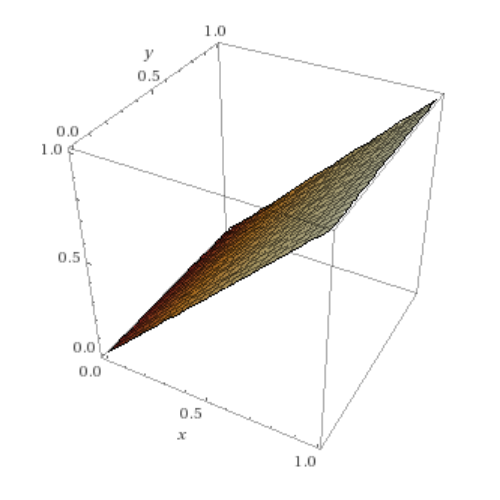
\includegraphics[width=5cm]{functionx}
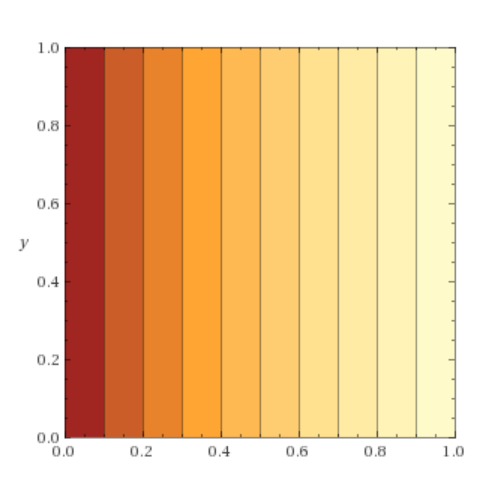
\includegraphics[width=5cm]{functionx2}
\end{figure}
\end{frame}

\begin{frame}
\frametitle{Príklad 2}
$$ F(x,y)=x*y*max(x,y)$$
Nespĺňa T2 (asociatívnosť).
\begin{figure}
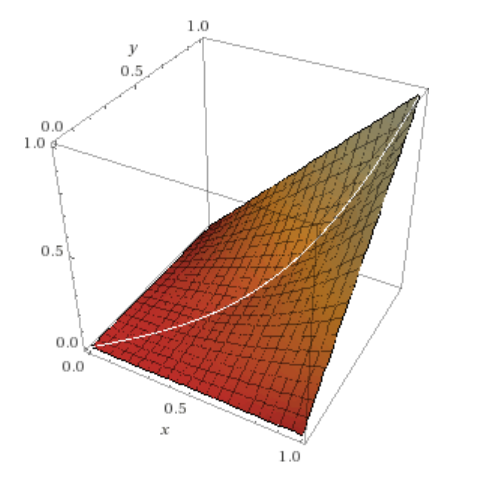
\includegraphics[width=5cm]{function3}
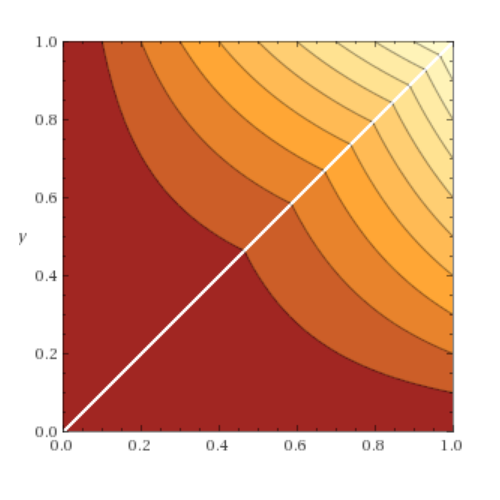
\includegraphics[width=5cm]{function32}
\end{figure}
\end{frame}


\begin{frame}
\frametitle{Príklad 3}
\[ F(x,y)=\begin{cases} 
      0.5 & ak (x, y) \in ]0,1[^2 \\
      min(x,y) & inak 
   \end{cases}
\]
Nespĺňa T3 (monotónnosť).
\begin{figure}
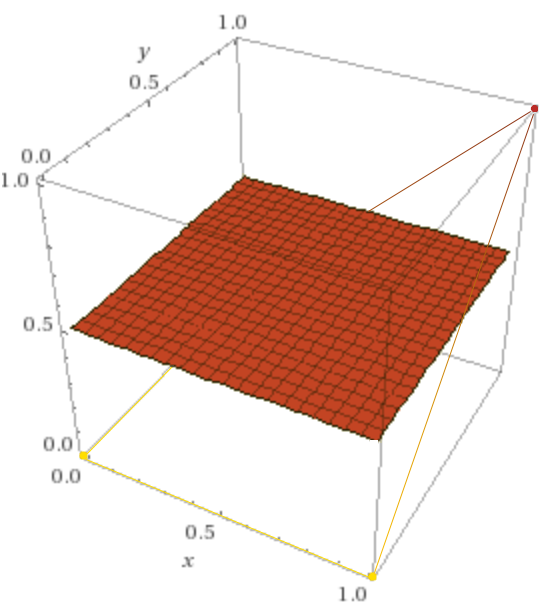
\includegraphics[width=4cm]{F3}
\end{figure}
\end{frame}


\begin{frame}
\frametitle{Príklad 4}
$$ F(x,y)=1/2$$
Nespĺňa T4 (okrajová podmienka).
\begin{figure}
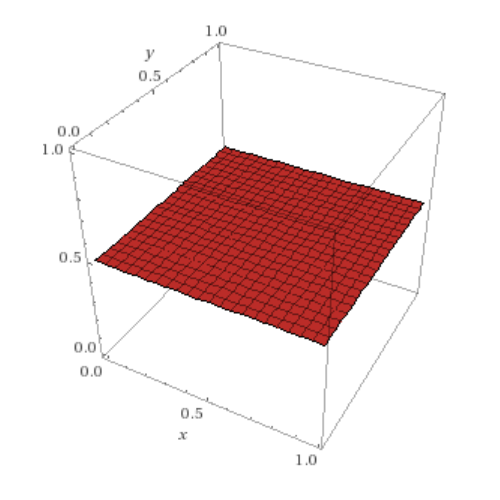
\includegraphics[width=5cm]{function12}
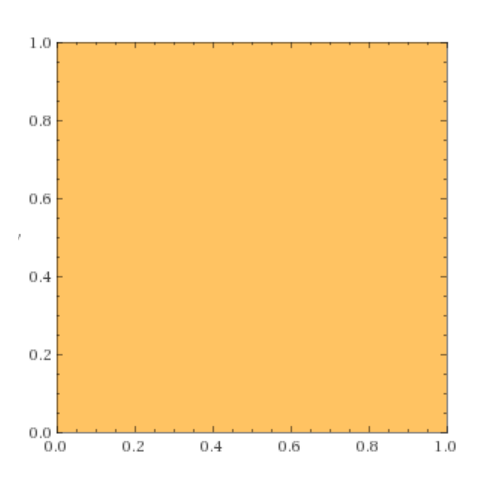
\includegraphics[width=5cm]{function122}
\end{figure}
\end{frame}

%MinimumTnorm
%ProductTnorm
%LukasiewiczTnorm
%DrasticTnorm





\begin{frame}
\frametitle{Základné t-normy}
\begin{columns}
\column{0.5\textwidth}
\begin{minipage}[c][0.4\textheight][c]{\linewidth}
  \centering
  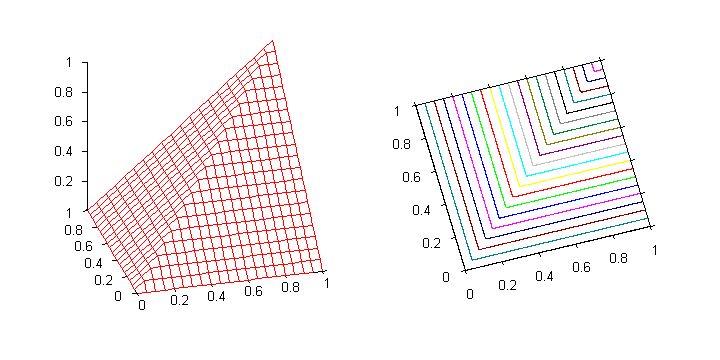
\includegraphics[width=0.9\linewidth]{MinimumTnorm}
  \captionof{figure}{Minimová}
\end{minipage}
\begin{minipage}[c][0.4\textheight][c]{\linewidth}
  \centering
  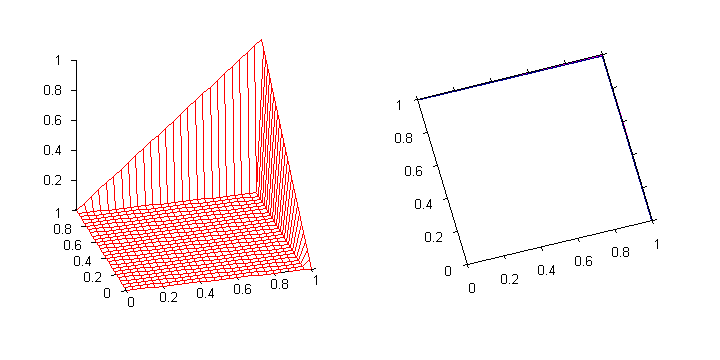
\includegraphics[width=0.9\linewidth]{DrasticTnorm}
  \captionof{figure}{Drastický Súčin}
\end{minipage}
\column{0.5\textwidth}
\begin{minipage}[c][0.4\textheight][c]{\linewidth}
$$ T_M(x,y)=\min(x,y)$$
\end{minipage}
\begin{minipage}[c][0.4\textheight][c]{\linewidth}
\footnotesize $$ T_D(x,y)=\begin{cases} \min(x,y),  &\mbox {ak
$\max(x,y)=1,$} \\0,  &\mbox
{inak.}\end{cases}$$
\end{minipage}
\end{columns}
\end{frame}

\begin{frame}
\frametitle{Základné t-normy}
\begin{columns}
\column{0.5\textwidth}
\begin{minipage}[c][0.4\textheight][c]{\linewidth}
  \centering
  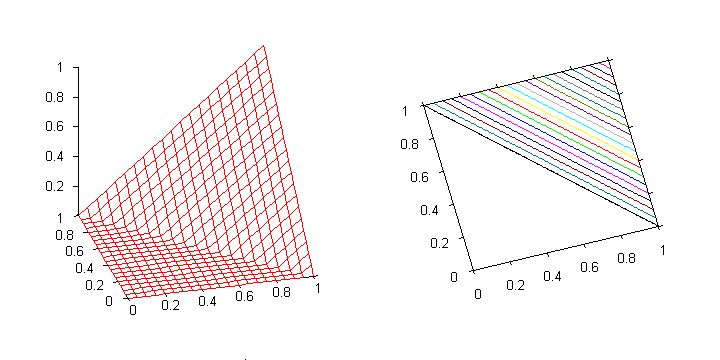
\includegraphics[width=0.9\linewidth]{LukasiewiczTnorm}
  \captionof{figure}{Lukasiewicz}
\end{minipage}
\begin{minipage}[c][0.4\textheight][c]{\linewidth}
  \centering
  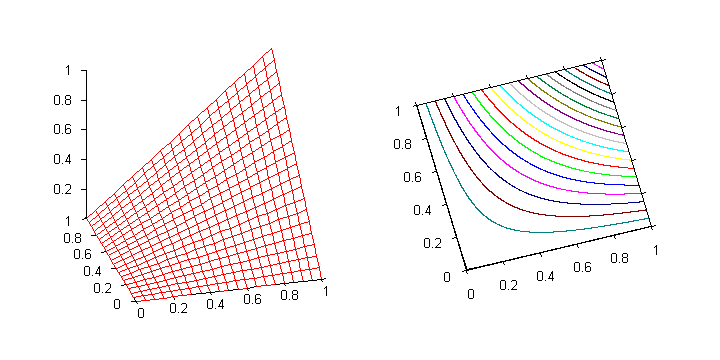
\includegraphics[width=0.9\linewidth]{ProductTnorm}
  \captionof{figure}{Súčinová}
\end{minipage}
\column{0.5\textwidth}
\begin{minipage}[c][0.4\textheight][c]{\linewidth}
$$ T_L(x,y)=\max(x+y-1,0)$$
\end{minipage}
\begin{minipage}[c][0.4\textheight][c]{\linewidth}
$$ T_P(x,y)=x.y$$
\end{minipage}
\end{columns}
\end{frame}


\begin{frame}
\frametitle{Vlastnosti}
\textbf{Poznámka:}
\begin{center}
Zrejme pre každú t-normu $T$ platí
$$ T(1,x)=T(x,1)=x,$$
$$ T(0,x)=T(x,0)=0.$$
\end{center}
\begin{definition}


\begin{itemize}
\item  Ak pre t-normy $T_1$ a $T_2$ je
pre každý bod $(x,y) \in [0,1]^2$ splnená nerovnosť
$T_1(x,y) \leq T_2(x,y),$ hovoríme, že $T_1$ je {\em slabšia} ako $T_2$,
alebo $T_2$ je {\em silnejšia} ako $T_1$ a píšeme $T_1\leq T_2$.
\item  Ak pre t-normy $T_1$ a $T_2$ platí, že $T_1 \leq T_2$ a
$T_1 \ne T_2,$ t.j. ak $T_1 \leq T_2$, ale $T_1(x_0,y_0) <
T_2(x_0,y_0)$ pre nejaký bod $(x_0,y_0) \in [0,1]^2$, tak $T_1<T_2$.
\end{itemize}
\end{definition}
\end{frame}

\begin{frame}
\frametitle{Sila}
\begin{columns}
\column{0.5\textwidth}
\begin{minipage}[c][0.4\textheight][c]{\linewidth}
  \centering
  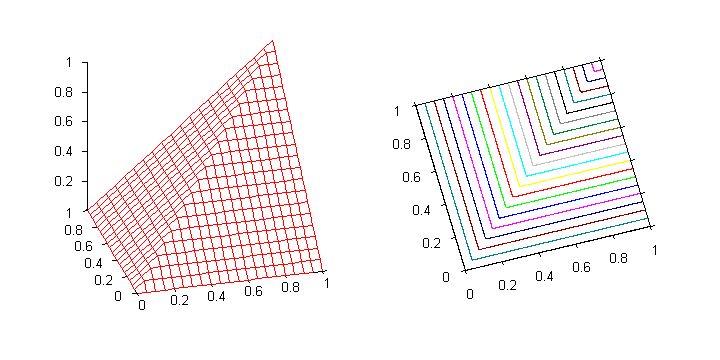
\includegraphics[width=0.9\linewidth]{MinimumTnorm}
  \captionof{figure}{Minimová}
\end{minipage}
\begin{minipage}[c][0.4\textheight][c]{\linewidth}
  \centering
  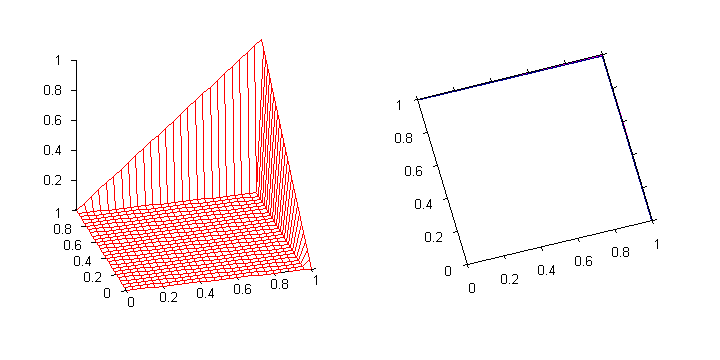
\includegraphics[width=0.9\linewidth]{DrasticTnorm}
  \captionof{figure}{Drastický Súčin}
\end{minipage}
\column{0.5\textwidth}
\begin{minipage}[c][0.4\textheight][c]{\linewidth}
  \centering
  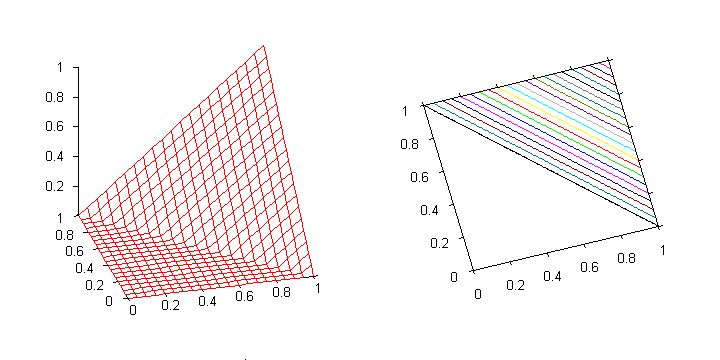
\includegraphics[width=0.9\linewidth]{LukasiewiczTnorm}
  \captionof{figure}{Lukasiewicz}
\end{minipage}
\begin{minipage}[c][0.4\textheight][c]{\linewidth}
  \centering
  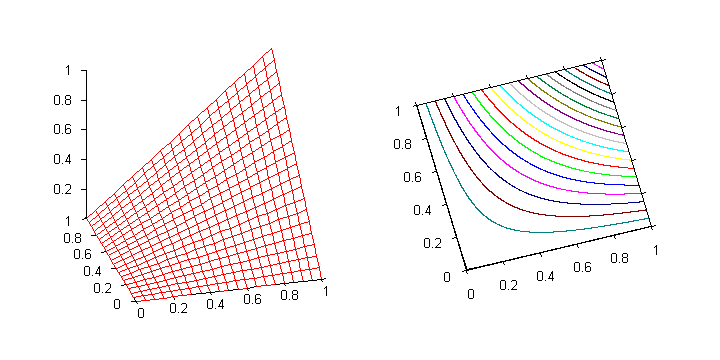
\includegraphics[width=0.9\linewidth]{ProductTnorm}
  \captionof{figure}{Súčinová}
\end{minipage}
\end{columns}
\end{frame}

\begin{frame}
\frametitle{Idempotentné prvky}
\begin{definition}
Význačné sú tie prvky, pre ktoré platí $T(a,a)=a.$ Nazývame ich
{\em idempotentné prvky t-normy} $T.$ Zrejme pre ľubovoľnú t-normu sú 0 a 1
idempotentné prvky. Preto ich nazývame {\em triviálnymi idempotentnými
prvkami.}
\end{definition}
\end{frame}


\begin{frame}
\begin{center}
{\bf Veta.} (Klement, Mesiar, Pap)
Minimová t-norma je jediná, pre ktorú je každý jej prvok $a \in [0,1]$
idempotentný, t.j.
$$( \forall a \in [0,1]: T(a,a)=a) \iff T=T_M.$$
\end{center}
\begin{center}
{\bf Dôkaz.} Ak pre t-normu $T$ očakávame $T(x,x)=x$ pre každé $x\in (0,1)$, potom keď $y\leq x<1$ monotónnosť (T3) implikuje 
$$y=T(y,y)\leq T(x,y)\leq min(x,y)=y$$
Spolu s komutativitou (T1) a okrajovou podmienkou (T4) získame $T=T_M$
\end{center}
Poznámka: Vysvetliť
\end{frame}

\begin{frame}
\frametitle{Algebraické vlastnosti}
\begin{itemize}
\item Archimedovská vlastnosť
\item Striktná monotónnosť
\item Ďeliteľ nuly
\item Nilpotentný prvok
\item Nilpotentnosť
\end{itemize}
\end{frame}

\begin{frame}
\frametitle{Archimedovská vlastnosť}
\begin{definition}
T-norma $T$ je {\em archimedovská,} ak pre všetky body $(x,y) \in ]0,1[^2$ existuje $n \in N$ také, že
$$ x_T^{(n)} < y.$$
\end{definition}
$$x_{T_M}^{(n)}=x, \hskip 3mm x_{T_P}^{(n)}= x^n, \hskip 3mm
x_{T_L}^{(n)}=
\max\{0, nx-n+1\}$$
\begin{small}
\textit{Poznámka: Odvodiť}\end{small}
\end{frame}

\begin{frame}
\frametitle{Vety}
%\begin{center}
{\bf Veta.}  (Klement, Mesiar, Pap)
Triangulárna norma T je archimedovská práve vtedy, ked pre každé $x \in ]0,1[$
je $$ \lim \limits_{n \rightarrow \infty} {x^{(n)}_T} = 0.$$

{\bf Veta.}  (Klement, Mesiar, Pap)
\begin{itemize}
\item Ak t-norma $T$ je archimedovská, tak pre každé $x
\in \hskip 1mm ]0,1[$ \hskip 1mm platí \hskip 1mm $ T(x,x) <~x$.
\item  Ak je t-norma $T$ spojitá sprava, potom je
archimedovská práve vtedy, keď pre každé $ x \in \hskip 1mm ]0,1[$ \hskip 1mm platí \hskip 1mm $
T(x,x) < x$.
\end{itemize}
%\end{center}
\end{frame}

\begin{frame}
\frametitle{Diagonály}
\begin{columns}
\column{0.5\textwidth}
\begin{minipage}[c][0.4\textheight][c]{\linewidth}
  \centering
  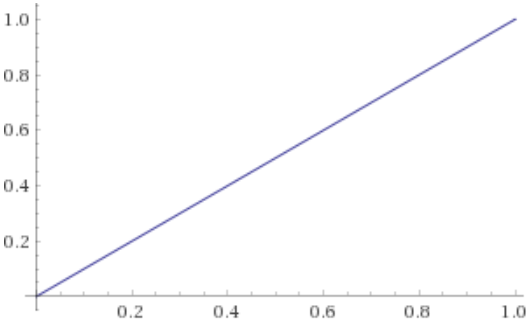
\includegraphics[width=0.8\linewidth]{minDiag}
  \captionof{figure}{Minimová t-norma}
\end{minipage}
\begin{minipage}[c][0.4\textheight][c]{\linewidth}
  \centering
  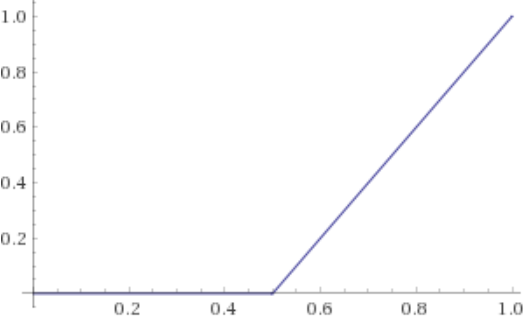
\includegraphics[width=0.8\linewidth]{lukaDiag}
  \captionof{figure}{Lakasiewiczova t-norma}
\end{minipage}
\column{0.5\textwidth}
\begin{minipage}[c][0.4\textheight][c]{\linewidth}
  \centering
  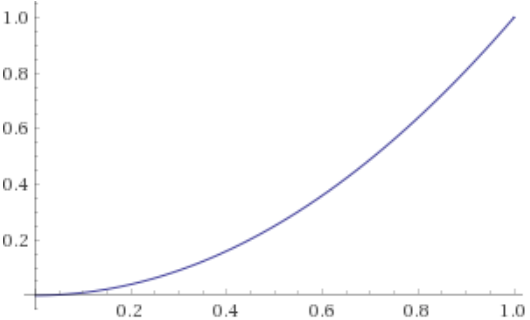
\includegraphics[width=0.8\linewidth]{prodDiag}
  \captionof{figure}{Súčinová t-norma}
\end{minipage}
\begin{minipage}[c][0.4\textheight][c]{\linewidth}
  \centering
  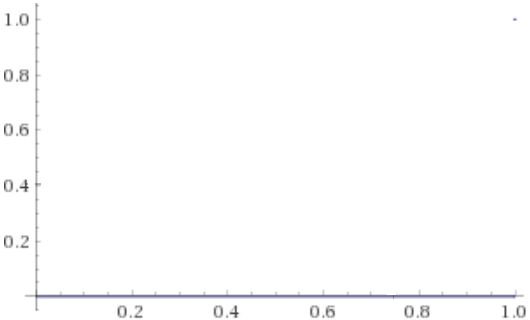
\includegraphics[width=0.8\linewidth]{drastDiag}
  \captionof{figure}{Drastický súčin}
\end{minipage}
\end{columns}
\end{frame}

\begin{frame}
\frametitle{Striktná monotónnosť}
\begin{itemize}
\item  Hovoríme, že t-norma $T$ je {\em striktne
monotónna}, ak
je rastúca na $]0,1]^2$ ako funkcia $ T:[0,1]^2 \rightarrow [0,1]$ alebo
ekvivaletne,
$$ \text {ak} \hskip 3mm x \in \hskip 1mm ]0,1] \hskip 3mm \text{a} \hskip 3mm y < z, \hskip 3mm \text {tak} \hskip 3mm T(x,y) < T(x,z). $$
\item  Hovoríme, že t-norma $T$ je {\em združene striktne
monotónna}, ak platí:
$$ \text{ak} \hskip 3mm  x < x'\hskip 3mm \text{a} \hskip 3mm y<y',
\hskip 3mm  \text{tak} \hskip 3mm   T(x,y)<T(x',y').$$
\item  Hovoríme, že t-norma $T$ je {\em striktná}, ak je spojitá a striktne monotónna.
\end{itemize}
\begin{small}\textit{Viď minimová}\end{small}
\end{frame}

\begin{frame}
\frametitle{Veta}
{\bf Veta.} (Klement, Mesiar, Pap)
%\begin{itemize}
%\item Triangulárna norma T je striktne monotónna práve vtedy, keď platí zákon
%o krátení, t.j. ak $T(x,y)=T(x,z)$  a  $x>0$, tak $y=z.$
Ak je t-norma T striktne monotónna, potom je aj združene striktne monotónna.
%\end{itemize}
\end{frame}

\begin{frame}
\frametitle{Dôkaz}
Striktne monotónna
$$ y<z \implies T(x,y)<T(x,z)$$
$$ x<z \implies T(x,y)<T(z,y)$$

Združene strikne monotónna
$$ x<x' \land y<y' \implies T(x,y)<T(x',y')$$
\end{frame}

\begin{frame}
\frametitle{Dôkaz}
Nech
$$ x<x' \land y<y' \implies T(x,y)<T(x',y)$$\pause
$$ \implies T(x,y')<T(x',y')$$\pause
$$ \implies T(x',y)<T(x',y')$$\pause
$$ \implies T(x,y)<T(x,y')$$\pause

Z toho vyplýva
$$ T(x,y)<T(x,y')<T(x',y')\implies T(x,y)<T(x',y')$$
\end{frame}

%\begin{frame}
%\frametitle{Delenie nulou?}
%\begin{figure}[H]
%  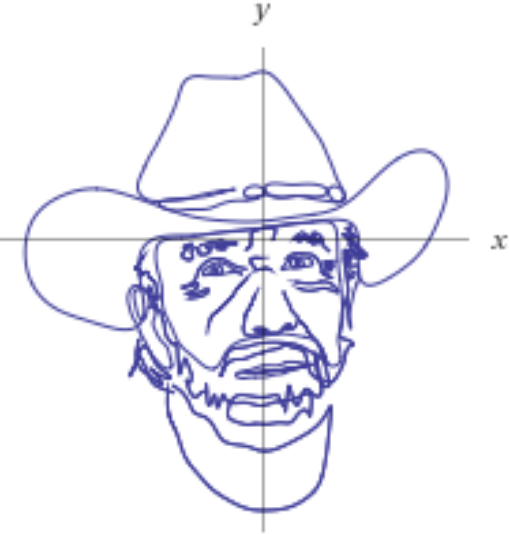
\includegraphics[width=0.4\linewidth]{norris}
%\end{figure}
%\end{frame}

\begin{frame}
\frametitle{Deliteľ nuly}
\begin{definition}
Prvok $x \in ]0,1[$ nazveme {\em deliteľ nuly} danej t-normy $T$, ak
existuje $y \in ]0,1[$ také, že $T(x,y) = 0.$\\
\end{definition}
Poznámka: Triangulárna norma bez deliteľov nuly sa nazýva {\em pozitívna.}
\end{frame}

\begin{frame}
\frametitle{Deliteľ nuly}
\begin{columns}
\column{0.5\textwidth}
\begin{minipage}[c][0.4\textheight][c]{\linewidth}
  \centering
  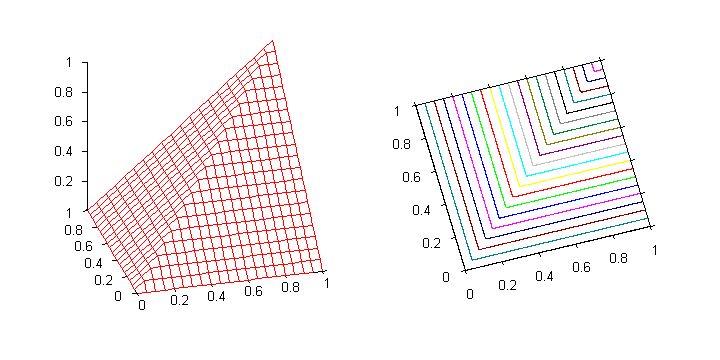
\includegraphics[width=0.9\linewidth]{MinimumTnorm}
  \captionof{figure}{Minimová}
\end{minipage}
\begin{minipage}[c][0.4\textheight][c]{\linewidth}
  \centering
  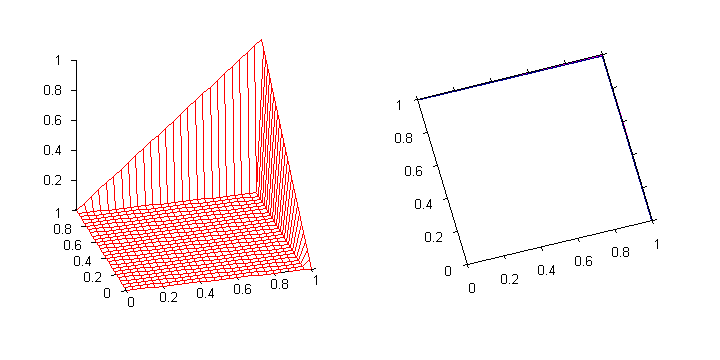
\includegraphics[width=0.9\linewidth]{DrasticTnorm}
  \captionof{figure}{Drastický Súčin}
\end{minipage}
\column{0.5\textwidth}
\begin{minipage}[c][0.4\textheight][c]{\linewidth}
  \centering
  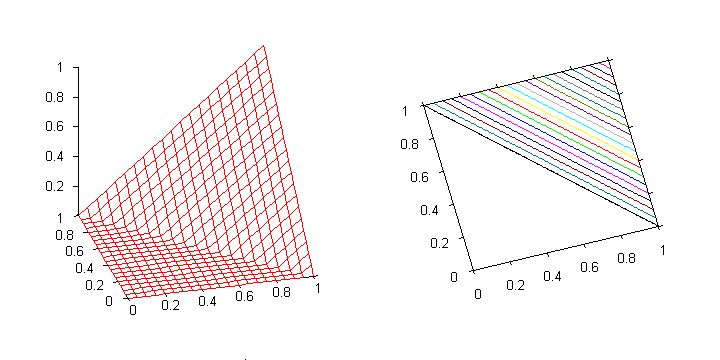
\includegraphics[width=0.9\linewidth]{LukasiewiczTnorm}
  \captionof{figure}{Lukasiewicz}
\end{minipage}
\begin{minipage}[c][0.4\textheight][c]{\linewidth}
  \centering
  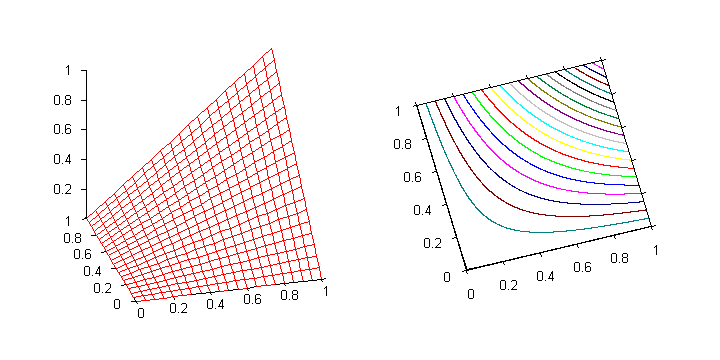
\includegraphics[width=0.9\linewidth]{ProductTnorm}
  \captionof{figure}{Súčinová}
\end{minipage}
\end{columns}
\end{frame}

\begin{frame}
\frametitle{Nilpotentné prvky}
\begin{definition}
Hovoríme, že $x \in ]0,1[$ je {\em nilpotentný prvok danej t-normy $T$}, ak existuje $n \in N$ také,
že $ x_T^{(n)} =0.$
\end{definition}
\begin{definition}
Hovoríme, že t-norma $T$ je {\em nilpotentná}, ak je spojitá a každé $x \in ]0,1[$ je jej nilpotentným prvkom.
\end{definition}
\end{frame}

%\begin{frame}
%\frametitle{Nilpotentnosť}
%\begin{definition}
%Hovoríme, že t-norma $T$ je {\em nilpotentná}, ak je spojitá a každé $x \in ]0,1[$ je jej nilpotentným prvkom.
%\end{definition}

%{\bf Veta.}  (Klement, Mesiar, Pap)
%Nech T je spojitá archimedovská t-norma. Potom nasledujúce tvrdenia
%sú ekvivalentné :
%\begin{itemize}
%\item T je nilpotentná.
%\item  Existuje aspoň jeden nilpotentný prvok danej
%t-normy T.
%\item T nie je striktná.
%\item  T má deliteľa nuly.
%\end{itemize}
%\end{frame}


\begin{frame}
\frametitle{Diagonály}
\begin{columns}
\column{0.5\textwidth}
\begin{minipage}[c][0.4\textheight][c]{\linewidth}
  \centering
  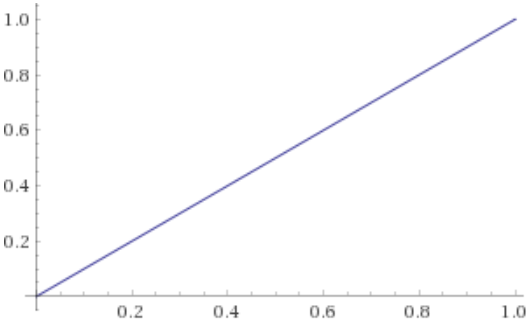
\includegraphics[width=0.8\linewidth]{minDiag}
  \captionof{figure}{Minimová t-norma}
\end{minipage}
\begin{minipage}[c][0.4\textheight][c]{\linewidth}
  \centering
  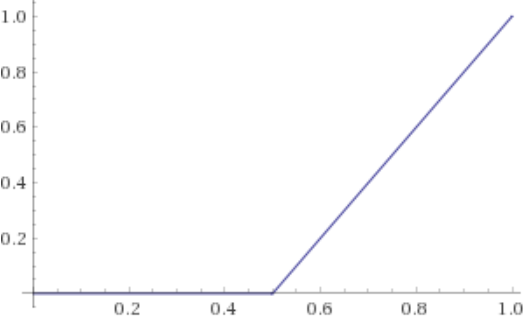
\includegraphics[width=0.8\linewidth]{lukaDiag}
  \captionof{figure}{Lakasiewiczova t-norma}
\end{minipage}
\column{0.5\textwidth}
\begin{minipage}[c][0.4\textheight][c]{\linewidth}
  \centering
  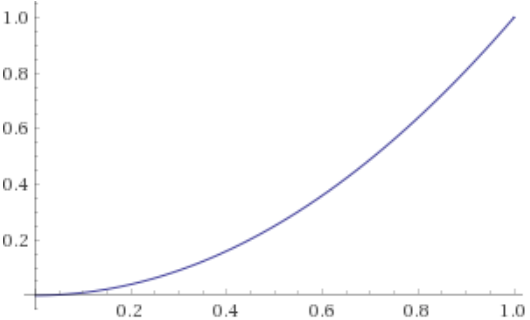
\includegraphics[width=0.8\linewidth]{prodDiag}
  \captionof{figure}{Súčinová t-norma}
\end{minipage}
\begin{minipage}[c][0.4\textheight][c]{\linewidth}
  \centering
  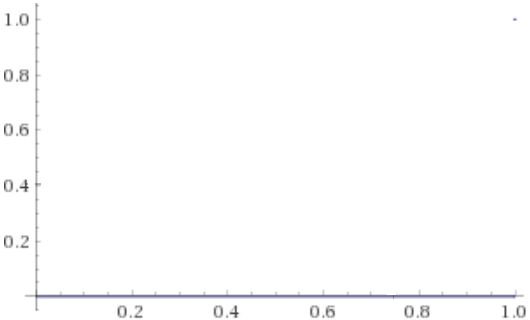
\includegraphics[width=0.8\linewidth]{drastDiag}
  \captionof{figure}{Drastický súčin}
\end{minipage}
\end{columns}
\end{frame}

\begin{frame}
\frametitle{Diagonály}
\begin{columns}
\column{0.5\textwidth}
\begin{minipage}[c][0.4\textheight][c]{\linewidth}
  \centering
  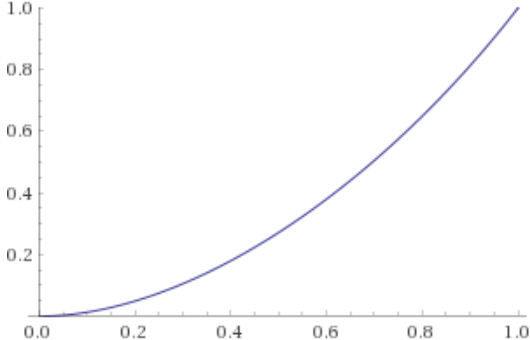
\includegraphics[width=0.7\linewidth]{FT/FT0_5-diag}
  \captionof{figure}{Príklad 1}
\end{minipage}
\begin{minipage}[c][0.4\textheight][c]{\linewidth}
  \centering
  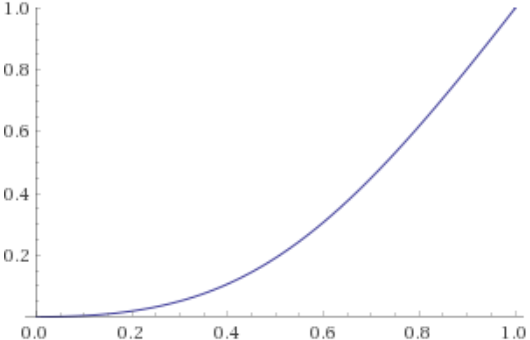
\includegraphics[width=0.7\linewidth]{FT/FT7-diag}
  \captionof{figure}{Príklad 2}
\end{minipage}
\column{0.5\textwidth}
\begin{minipage}[c][0.4\textheight][c]{\linewidth}
  \centering
  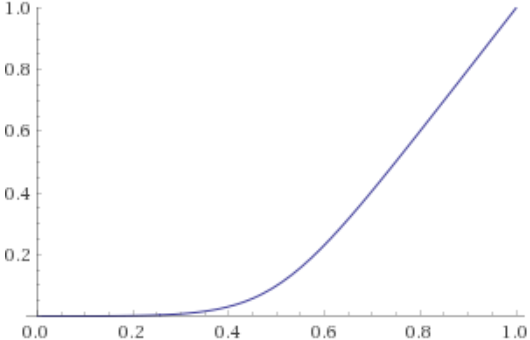
\includegraphics[width=0.7\linewidth]{FT/FT750-diag}
  \captionof{figure}{Príklad 3}
\end{minipage}
\begin{minipage}[c][0.4\textheight][c]{\linewidth}
  \centering
  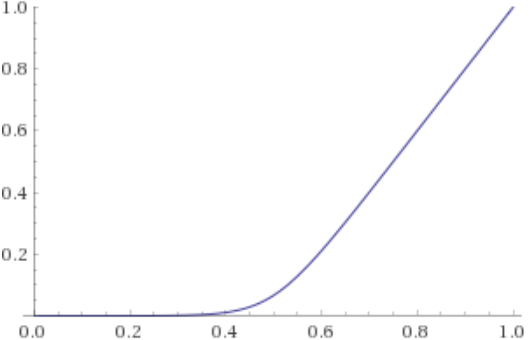
\includegraphics[width=0.7\linewidth]{FT/FT30000-diag}
  \captionof{figure}{Príklad 4}
\end{minipage}
\end{columns}
\end{frame}




\begin{frame}
\frametitle{Parametrické t-normy}
\begin{itemize}
\item Schweizer–Sklar t-normy
\item Frankove t-normy
\item ...
\end{itemize}
\end{frame}


\begin{frame}
\frametitle{Schweizer–Sklar t-normy}
\[ T_P^{SS}(x,y)=\begin{cases} 
      T_{min}(x,y) & p = -\infty \\
      (x^p + y^p -1)^{\frac{1}{p}} & -\infty < p < 0 \\
      T_{prod}(x,y) & p = 0 \\
      (max(0,x^p + y^p -1))^{\frac{1}{p}} & 0 < p < \infty \\
      T_D(x,y) & p = \infty 
   \end{cases}
\]
\end{frame}
\begin{frame}
\frametitle{Vlastnosti}
\begin{itemize}
    \item Archimedovská iba pre $p > -\infty$
    \item Spojitá iba pre $p < +\infty$
    \item Striktná iba pre $-\infty < p \leq 0$
    \item Nilpotentná iba pre $0 < p < +\infty$ (pre $p = 1$  $T_{Luk}$).
\end{itemize}
\end{frame}

%MinimumTnorm
%ProductTnorm
%LukasiewiczTnorm
%DrasticTnorm


\begin{frame}
\frametitle{Schweizer–Sklar t-normy}
\begin{columns}
\column{0.5\textwidth}
\begin{minipage}[c][0.4\textheight][c]{\linewidth}
  \centering
  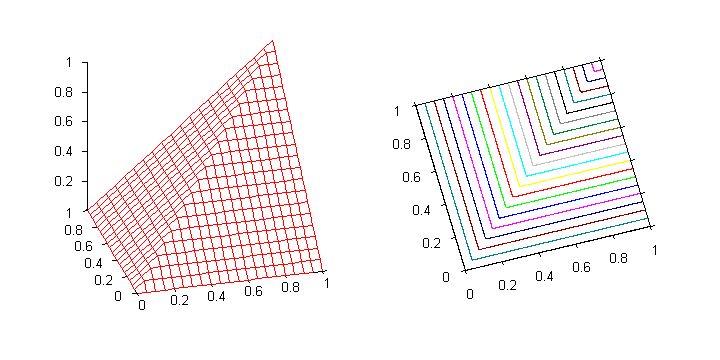
\includegraphics[width=1.1\linewidth]{MinimumTnorm}
\end{minipage}
\begin{minipage}[c][0.4\textheight][c]{\linewidth}
  \centering
  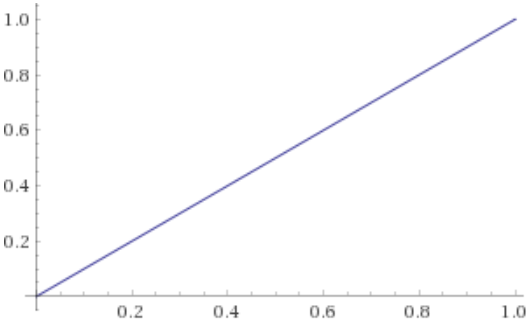
\includegraphics[width=0.7\linewidth]{minDiag}
  \captionof{figure}{$T_{MIN}$:Schweizer–Sklar pre p = $-\infty$}
\end{minipage}
\column{0.5\textwidth}
\begin{minipage}[c][0.4\textheight][c]{\linewidth}
  \centering
  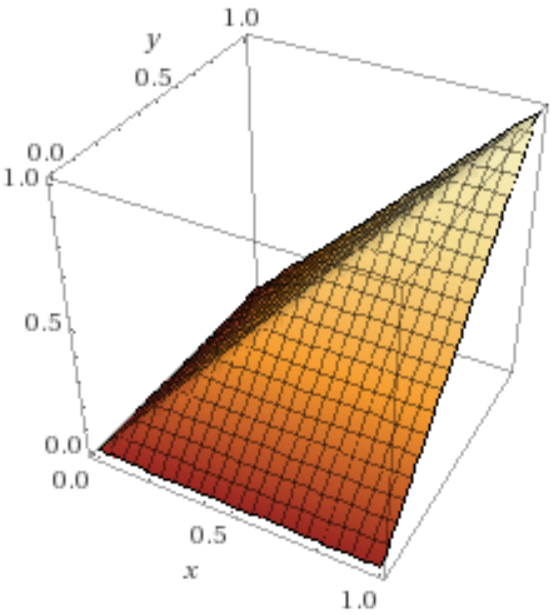
\includegraphics[width=0.5\linewidth]{SS-19000}
\end{minipage}
\begin{minipage}[c][0.4\textheight][c]{\linewidth}
  \centering
  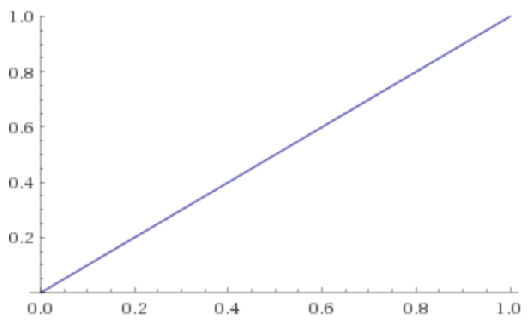
\includegraphics[width=0.7\linewidth]{SS-19000-diag}
  \captionof{figure}{Schweizer–Sklar pre p = -19000}
\end{minipage}
\end{columns}
\end{frame}


\begin{frame}
\frametitle{Schweizer–Sklar t-normy}
\begin{columns}
\column{0.5\textwidth}
\begin{minipage}[c][0.4\textheight][c]{\linewidth}
  \centering
  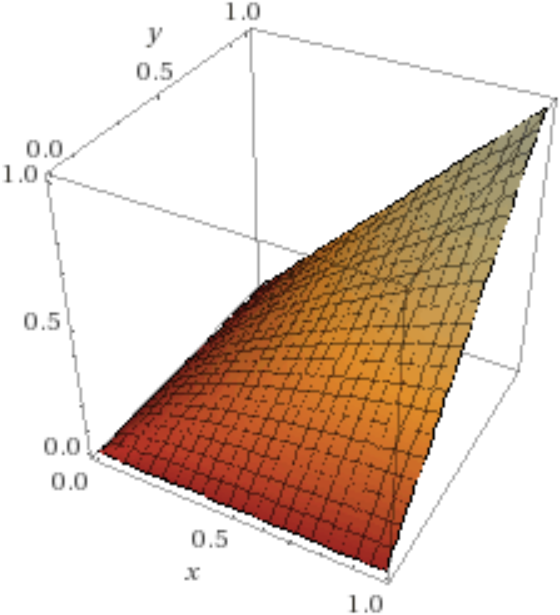
\includegraphics[width=0.5\linewidth]{SS-0-5}
\end{minipage}
\begin{minipage}[c][0.4\textheight][c]{\linewidth}
  \centering
  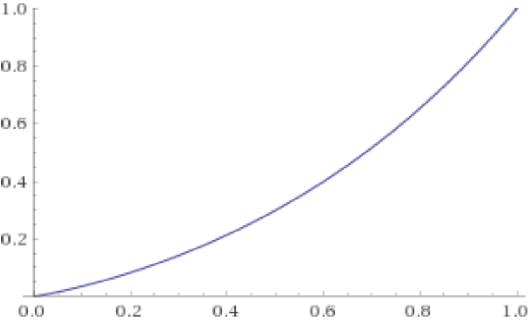
\includegraphics[width=0.7\linewidth]{SS-0-5-diag}
  \captionof{figure}{Schweizer–Sklar pre p = -0.5}
\end{minipage}
\column{0.5\textwidth}
\begin{minipage}[c][0.4\textheight][c]{\linewidth}
  \centering
  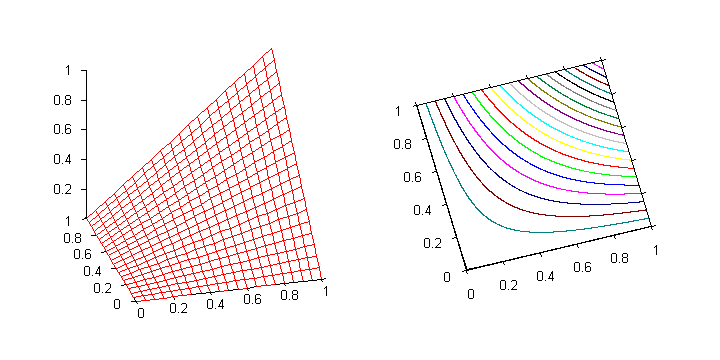
\includegraphics[width=1.1\linewidth]{ProductTnorm}
\end{minipage}
\begin{minipage}[c][0.4\textheight][c]{\linewidth}
  \centering
  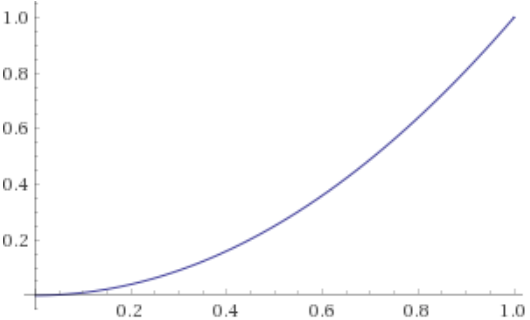
\includegraphics[width=0.7\linewidth]{prodDiag}
  \captionof{figure}{$T_{prod}$:Schweizer–Sklar pre p = 0}
\end{minipage}
\end{columns}
\end{frame}

\begin{frame}
\frametitle{Schweizer–Sklar t-normy}
\begin{columns}
\column{0.5\textwidth}
\begin{minipage}[c][0.4\textheight][c]{\linewidth}
  \centering
  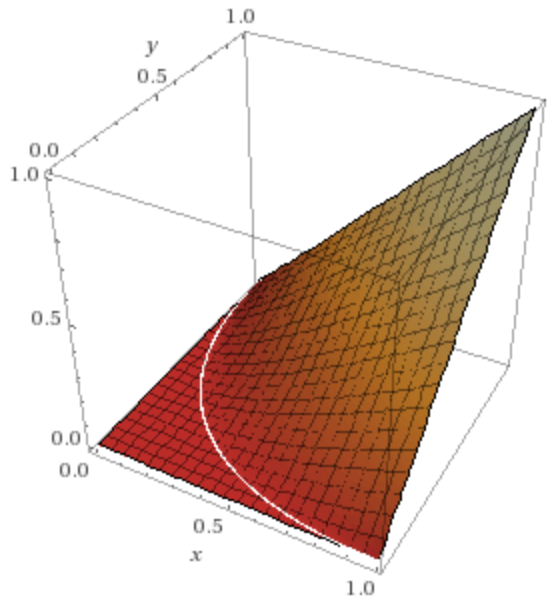
\includegraphics[width=0.5\linewidth]{SS0_2}
\end{minipage}
\begin{minipage}[c][0.4\textheight][c]{\linewidth}
  \centering
  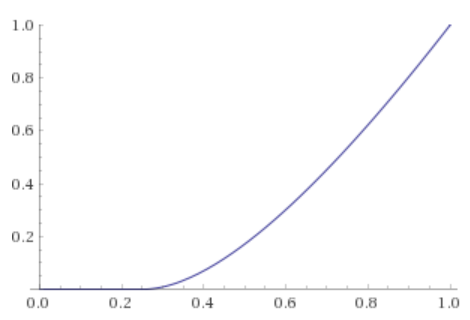
\includegraphics[width=0.7\linewidth]{SS0_2-diag}
  \captionof{figure}{Schweizer–Sklar pre p = 0.2}
\end{minipage}
\column{0.5\textwidth}
\begin{minipage}[c][0.4\textheight][c]{\linewidth}
  \centering
  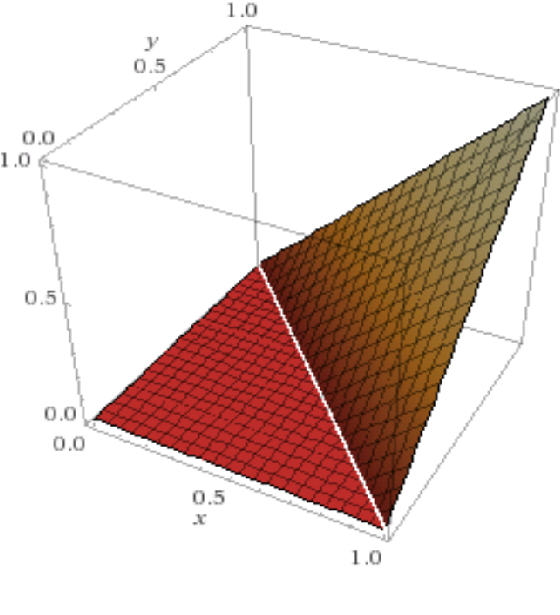
\includegraphics[width=0.5\linewidth]{SS1-luka}
\end{minipage}
\begin{minipage}[c][0.4\textheight][c]{\linewidth}
  \centering
  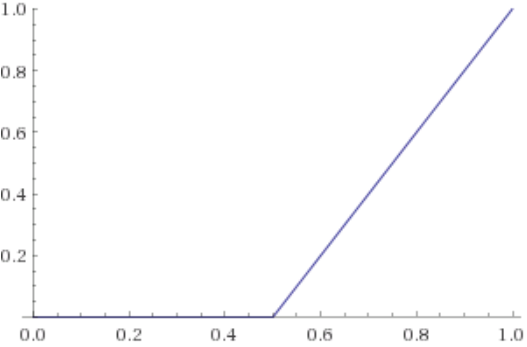
\includegraphics[width=0.7\linewidth]{SS1-luka-diag}
  \captionof{figure}{$T_{Luk}$Schweizer–Sklar pre p = 1}
\end{minipage}
\end{columns}
\end{frame}

\begin{frame}
\frametitle{Schweizer–Sklar t-normy}
\begin{columns}
\column{0.5\textwidth}
\begin{minipage}[c][0.4\textheight][c]{\linewidth}
  \centering
  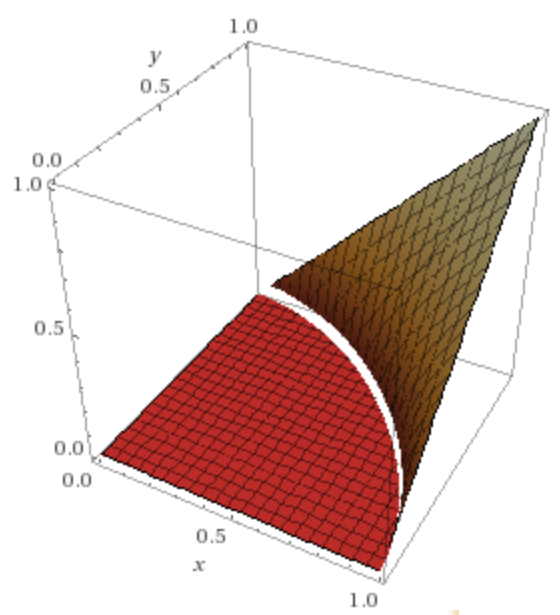
\includegraphics[width=0.5\linewidth]{SS1-7}
\end{minipage}
\begin{minipage}[c][0.4\textheight][c]{\linewidth}
  \centering
  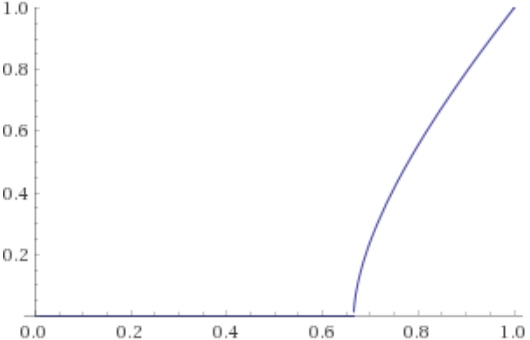
\includegraphics[width=0.7\linewidth]{SS1_7-diag}
  \captionof{figure}{Schweizer–Sklar pre p = 1.7}
\end{minipage}
\column{0.5\textwidth}
\begin{minipage}[c][0.4\textheight][c]{\linewidth}
  \centering
  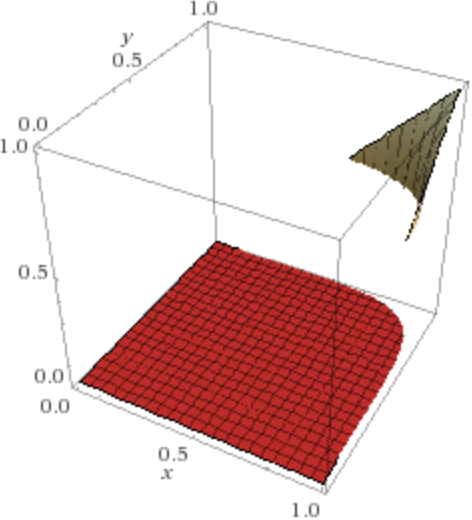
\includegraphics[width=0.5\linewidth]{SS7}
\end{minipage}
\begin{minipage}[c][0.4\textheight][c]{\linewidth}
  \centering
  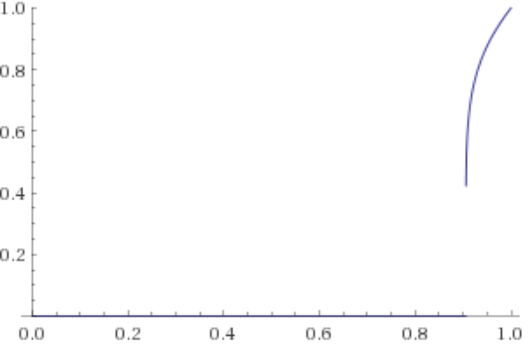
\includegraphics[width=0.7\linewidth]{SS7-diag}
  \captionof{figure}{Schweizer–Sklar pre p = 7}
\end{minipage}\end{columns}
\end{frame}

\begin{frame}
\frametitle{Schweizer–Sklar t-normy}
\begin{columns}
\column{0.5\textwidth}
\begin{minipage}[c][0.4\textheight][c]{\linewidth}
  \centering
  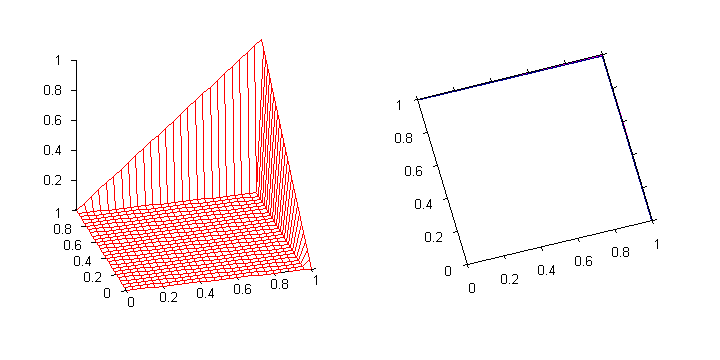
\includegraphics[width=1.1\linewidth]{DrasticTnorm}
\end{minipage}
\begin{minipage}[c][0.4\textheight][c]{\linewidth}
  \centering
  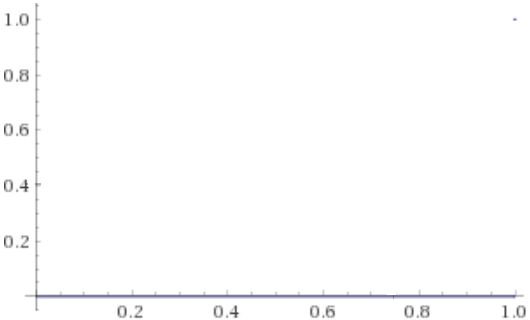
\includegraphics[width=0.7\linewidth]{drastDiag}
  \captionof{figure}{$T_D$:Schweizer–Sklar pre p = $\infty$}
\end{minipage}
\column{0.5\textwidth}
\end{columns}
\end{frame}

\begin{frame}
\frametitle{Frankove t-normy}
Pre $0 \leq p \leq +\infty$:
\[ T_P^{F}(x,y)=\begin{cases} 
      T_{min}(x,y) & p = 0 \\
      T_{prod} & p = 1 \\
      T_{Luk}(x,y) & p = +\infty \\
      \log_p(1+\frac{(p^x-1)(p^y-1)}{p-1}) & inak
   \end{cases}
\]
\end{frame}



\begin{frame}
\frametitle{Frankove t-normy}
\begin{columns}
\column{0.5\textwidth}
\begin{minipage}[c][0.4\textheight][c]{\linewidth}
  \centering
  \includegraphics[width=1.1\linewidth]{MinimumTnorm}
\end{minipage}
\begin{minipage}[c][0.4\textheight][c]{\linewidth}
  \centering
  \includegraphics[width=0.7\linewidth]{minDiag}
  \captionof{figure}{$T_{min}$:Frank pre p = 0}
\end{minipage}
\column{0.5\textwidth}
\begin{minipage}[c][0.4\textheight][c]{\linewidth}
  \centering
  \includegraphics[width=0.5\linewidth]{FT/FT0_5}
\end{minipage}
\begin{minipage}[c][0.4\textheight][c]{\linewidth}
  \centering
  \includegraphics[width=0.7\linewidth]{FT/FT0_5-diag}
  \captionof{figure}{Frank pre p = 0.5}
\end{minipage}
\end{columns}
\end{frame}


\begin{frame}
\frametitle{Frankove t-normy}
\begin{columns}
\column{0.5\textwidth}
\begin{minipage}[c][0.4\textheight][c]{\linewidth}
  \centering
  \includegraphics[width=1.1\linewidth]{ProductTnorm}
\end{minipage}
\begin{minipage}[c][0.4\textheight][c]{\linewidth}
  \centering
  \includegraphics[width=0.7\linewidth]{prodDiag}
  \captionof{figure}{$T_{prod}$:Frank pre p = 1}
\end{minipage}
\column{0.5\textwidth}
\begin{minipage}[c][0.4\textheight][c]{\linewidth}
  \centering
  \includegraphics[width=0.5\linewidth]{FT/FT7}
\end{minipage}
\begin{minipage}[c][0.4\textheight][c]{\linewidth}
  \centering
  \includegraphics[width=0.7\linewidth]{FT/FT7-diag}
  \captionof{figure}{Frank pre p = 7}
\end{minipage}
\end{columns}
\end{frame}

\begin{frame}
\frametitle{Frankove t-normy}
\begin{columns}
\column{0.5\textwidth}
\begin{minipage}[c][0.4\textheight][c]{\linewidth}
  \centering
  \includegraphics[width=0.5\linewidth]{FT/FT30000}
\end{minipage}
\begin{minipage}[c][0.4\textheight][c]{\linewidth}
  \centering
  \includegraphics[width=0.7\linewidth]{FT/FT30000-diag}
  \captionof{figure}{Frank pre p = 30000}
\end{minipage}
\column{0.5\textwidth}
\begin{minipage}[c][0.4\textheight][c]{\linewidth}
  \centering
  \includegraphics[width=1.1\linewidth]{LukasiewiczTnorm}
\end{minipage}
\begin{minipage}[c][0.4\textheight][c]{\linewidth}
  \centering
  \includegraphics[width=0.7\linewidth]{lukaDiag}
  \captionof{figure}{$T_{Luk}$:Frank pre p = $\infty$}
\end{minipage}
\end{columns}
\end{frame}

\end{document}